% Relatorio - Topicos em IA (UFPI - CCN - DC) - Questoes 01, 02 e 03.
% Classe article, fonte Times, margens ABNT, citacoes abntex2cite (autor-data).
% Compile com: ./compile.sh   ou   make build

\documentclass[12pt,a4paper]{article}

\usepackage[T1]{fontenc}
\usepackage[utf8]{inputenc}
\usepackage[brazil]{babel}
\usepackage{mathptmx}
\usepackage[top=3cm,bottom=2cm,left=3cm,right=2cm]{geometry}
\usepackage{indentfirst}
\usepackage{setspace}
\usepackage{graphicx}
\usepackage{booktabs}
\usepackage{tabularx}
\usepackage{array}
\usepackage{ragged2e}
\usepackage{amsmath}
\usepackage{amssymb}
\usepackage{enumitem}
\usepackage{listings}
\usepackage{xcolor}
\usepackage{microtype}
\usepackage{csquotes}
\usepackage{titlesec}
\usepackage{fancyhdr}
\usepackage[colorlinks=true,urlcolor=blue,linkcolor=black,citecolor=blue]{hyperref}
\usepackage[alf]{abntex2cite}

\graphicspath{{figures/}}

\onehalfspacing
\setlength{\parindent}{1.25cm}
\renewcommand{\arraystretch}{1.3}

\titleformat{\section}{\normalfont\bfseries}{\thesection.}{0.5em}{\MakeUppercase}
\titleformat{\subsection}{\normalfont\bfseries}{\thesubsection}{0.5em}{}

\pagestyle{plain}

\definecolor{cinzacodigo}{gray}{0.95}
\definecolor{comentario}{rgb}{0.30,0.45,0.30}
\definecolor{palavrachave}{rgb}{0.10,0.10,0.60}

\lstset{
  basicstyle=\ttfamily\small,
  backgroundcolor=\color{cinzacodigo},
  commentstyle=\color{comentario},
  keywordstyle=\color{palavrachave}\bfseries,
  showstringspaces=false,
  breaklines=true,
  frame=single,
  framesep=5pt,
  columns=fullflexible,
  literate=
    {á}{{\'a}}1 {à}{{\`a}}1 {â}{{\^a}}1 {ã}{{\~a}}1 {ä}{{\"a}}1
    {é}{{\'e}}1 {ê}{{\^e}}1 {í}{{\'i}}1 {ó}{{\'o}}1 {ô}{{\^o}}1
    {õ}{{\~o}}1 {ú}{{\'u}}1 {ç}{{\c c}}1
    {Á}{{\'A}}1 {Â}{{\^A}}1 {Ã}{{\~A}}1 {É}{{\'E}}1 {Ê}{{\^E}}1
    {Í}{{\'I}}1 {Ó}{{\'O}}1 {Ô}{{\^O}}1 {Õ}{{\~O}}1 {Ú}{{\'U}}1 {Ç}{{\c C}}1,
}

\begin{document}

\thispagestyle{empty}

\begin{center}
  \textbf{UNIVERSIDADE FEDERAL DO PIAUÍ (UFPI)}\\
  \textbf{CENTRO DE CIÊNCIAS DA NATUREZA (CCN)}\\
  \textbf{DEPARTAMENTO DE COMPUTAÇÃO (DC)}\\[0.3em]
  Disciplina: Tópicos em Inteligência Artificial\\
  Professor: Raimundo Santos Moura \quad--\quad Período: 2026.1
\end{center}

\vspace{3.5cm}

\begin{center}
  {\Large \textbf{Pré-Treino e Pós-Treino de Modelos de Linguagem para o Domínio Público Piauiense}}\\[0.8em]
  {\large Relatório das Questões 01 (Pré-Treino Continuado), 02 (SFT) e 03 (LoRA/QLoRA)}
\end{center}

\vspace{2.5cm}

\begin{center}
\begin{tabularx}{0.8\textwidth}{|>{\RaggedRight\arraybackslash}X|}
  \hline
  \textbf{Modelo base:} Qwen2.5-0.5B (494M parâmetros)\\
  \hline
  \textbf{Datasets:} DOMPI-2025 (Diário Oficial dos Municípios do Piauí) e docentesDC (materiais dos docentes do DC/UFPI)\\
  \hline
  \textbf{Ambiente de treino:} Kaggle (1 GPU NVIDIA T4, 16~GB)\\
  \hline
\end{tabularx}
\end{center}

\vspace{3cm}

\begin{center}
  \textbf{Autores}\\[0.3em]
  Allycia \quad\textbar\quad Heverton \quad\textbar\quad Izaías \quad\textbar\quad Oscar
\end{center}

\vfill

\begin{center}
  Teresina -- PI\\
  2026
\end{center}


\newpage

\section{Introdução}

Modelos de linguagem de grande porte (\textit{Large Language Models}, LLMs) são
pré-treinados sobre vastos corpora de texto de propósito geral. Embora isso lhes
confira fluência ampla, o conhecimento adquirido tende a ser raso em domínios
especializados e em variedades regionais da língua, pouco representados nos dados
de origem. Adaptar esses modelos a um domínio específico, com custo computacional
acessível, é um problema central tanto na pesquisa quanto na aplicação prática de
Processamento de Linguagem Natural~\cite{gururangan2020dont}.

Este relatório documenta três experimentos de adaptação do modelo
\texttt{Qwen2.5-0.5B}~\cite{qwen2025} ao domínio público piauiense, conduzidos no
âmbito da disciplina de Tópicos em Inteligência Artificial. Cada experimento
corresponde a uma questão do trabalho e a uma técnica distinta de treinamento:

\begin{itemize}[leftmargin=2.2em]
  \item \textbf{Questão 01 -- Pré-Treino Continuado.} Adaptação não supervisionada
        do modelo ao corpus DOMPI-2025 (Diário Oficial dos Municípios do Piauí),
        avaliando a qualidade da modelagem de linguagem antes e depois do treino.
  \item \textbf{Questão 02 -- Pós-Treino com SFT.} Ajuste fino supervisionado
        (\textit{Supervised Fine-Tuning}) sobre pares de pergunta e resposta
        gerados a partir do dataset docentesDC, atualizando todos os parâmetros do
        modelo.
  \item \textbf{Questão 03 -- Pós-Treino com LoRA/QLoRA.} Repetição do experimento
        anterior por meio de adaptação de baixo posto (\textit{Low-Rank
        Adaptation}), que atualiza menos de 1\% dos parâmetros, comparando custo e
        qualidade frente ao ajuste fino completo.
\end{itemize}

As três técnicas são avaliadas pelas mesmas métricas quantitativas de modelagem de
linguagem: perplexidade, entropia cruzada e acurácia de previsão de
tokens~\cite{jelinek1977perplexity}. A hipótese geral é que o treinamento, em todas
as suas formas, reduz a incerteza do modelo sobre o texto do domínio e melhora sua
capacidade de previsão.

\subsection{Estado dos experimentos e escopo do relatório}

A Questão 01 foi executada de ponta a ponta em uma GPU NVIDIA T4 (Kaggle), com
resultados completos antes e depois do treino. As Questões 02 e 03 tiveram a
geração dos dados, o carregamento dos modelos e a avaliação \textit{baseline} (antes
do treino) concluídos; o laço de treinamento, contudo, foi interrompido em uma
tentativa de execução local por restrição de tempo de hardware. Por essa razão, este
relatório apresenta para as Questões 02 e 03 a metodologia completa e os resultados
\textit{baseline} reais já coletados, deixando as métricas pós-treino sinalizadas
como \emph{em andamento}. Essa decisão preserva a honestidade dos números
reportados: nenhuma métrica é estimada ou fabricada. A
Seção~\ref{sec:consideracoes} detalha o caminho de conclusão dessas duas questões.

\section{Fundamentação Teórica}

\subsection{Modelos de linguagem e o objetivo de pré-treino}

Um modelo de linguagem autorregressivo, baseado na arquitetura
\textit{Transformer}~\cite{vaswani2017attention}, estima a probabilidade do próximo
token $x_t$ dado o contexto anterior, $P(x_t \mid x_{<t})$. O treinamento minimiza a
entropia cruzada média entre a distribuição prevista e o token observado:

\begin{equation}
  \mathcal{L} = -\frac{1}{N} \sum_{t=1}^{N} \log P(x_t \mid x_{<t}),
  \label{eq:entropia}
\end{equation}

\noindent onde $N$ é o número de tokens. O \texttt{Qwen2.5-0.5B} adotado neste
trabalho possui 494 milhões de parâmetros, 24 camadas, dimensão oculta de 896 e
vocabulário de 151.936 tokens~\cite{qwen2025}.

\subsection{Pré-treino continuado (\textit{continued pretraining})}

O pré-treino continuado consiste em prosseguir o treino não supervisionado de um
modelo já pré-treinado sobre um corpus de um domínio-alvo, usando o mesmo objetivo
da Equação~\ref{eq:entropia}. A técnica adapta o modelo ao vocabulário, ao estilo e
às regularidades estatísticas do domínio sem necessidade de rótulos, e é
reconhecidamente eficaz para domínios especializados~\cite{gururangan2020dont}. É a
abordagem da Questão 01.

\subsection{Pós-treino: ajuste fino supervisionado (SFT)}

O \textit{Supervised Fine-Tuning} (SFT) treina o modelo sobre pares de instrução e
resposta, ensinando-o a seguir comandos e a responder no formato
desejado~\cite{ouyang2022instructgpt}. Os exemplos seguem tipicamente um molde de
prompt como o do \textit{Stanford Alpaca}~\cite{taori2023alpaca}, com campos de
instrução, entrada opcional e resposta. No SFT clássico (Questão 02), todos os
parâmetros do modelo são atualizados, o que oferece máxima capacidade de adaptação
ao custo de elevada demanda de memória e tempo.

\subsection{Adaptação eficiente: LoRA e QLoRA}

A \textit{Low-Rank Adaptation} (LoRA)~\cite{hu2022lora} congela os pesos originais
$W_0$ e aprende apenas um par de matrizes de baixo posto $A$ e $B$, de modo que a
atualização efetiva seja $W_0 + BA$, com $\mathrm{posto}(BA) = r \ll d$. Como apenas
$A$ e $B$ são treinados, o número de parâmetros atualizados cai em ordens de
grandeza, reduzindo memória e tempo sem alterar a arquitetura na inferência.

O QLoRA~\cite{dettmers2023qlora} estende a ideia carregando o modelo base
\emph{quantizado} em 4 bits (formato NF4) e aplicando os adaptadores LoRA sobre essa
representação comprimida~\cite{dettmers2022llmint8}. Isso permite ajustar modelos em
GPUs modestas. Ambas as técnicas são disponibilizadas pela biblioteca
PEFT~\cite{peft2022} e correspondem à Questão 03.

\subsection{Métricas de avaliação}
\label{sec:metricas}

As três questões usam o mesmo conjunto de métricas, calculadas sobre um conjunto de
avaliação reservado (\textit{held-out}):

\begin{itemize}[leftmargin=2.2em]
  \item \textbf{Entropia cruzada:} a perda média da Equação~\ref{eq:entropia};
        quanto menor, melhor o ajuste do modelo ao texto.
  \item \textbf{Perplexidade:} o exponencial da entropia cruzada,
        $\mathrm{PPL} = e^{\mathcal{L}}$~\cite{jelinek1977perplexity}. Interpreta-se
        como o número médio de opções entre as quais o modelo hesita por token; uma
        perplexidade próxima de 1 indica previsão quase determinística.
  \item \textbf{Acurácia de previsão de tokens:} a fração de tokens em que o token de
        maior probabilidade (\textit{argmax}) coincide com o token real.
\end{itemize}

\section{Metodologia Geral}
\label{sec:metodologia}

\subsection{Conjuntos de dados}

\paragraph{DOMPI-2025 (Questão 01).} O corpus DOMPI-2025~\cite{dataset_dompi2025}
reúne publicações do Diário Oficial dos Municípios do Piauí (DOM-PI) referentes a
2025, distribuídas em 12 territórios de desenvolvimento do estado. O texto foi
extraído dos PDFs originais com PaddleOCR, Docling e PyMuPDF, totalizando 77.337
documentos brutos. Trata-se de linguagem jurídico-administrativa: portarias,
decretos, extratos de contrato, editais de licitação e relatórios fiscais.

\paragraph{docentesDC (Questões 02 e 03).} O dataset
docentesDC~\cite{dataset_docentesdc} contém materiais acadêmicos (slides, notas de
aula, fragmentos de código e artigos) de 19 professores do Departamento de
Computação da UFPI, em 13.762 registros com os campos \texttt{text} e
\texttt{nome\_professor}. O conteúdo é heterogêneo e ruidoso: além de texto em
português extraído de slides, há artigos científicos em inglês fatiados em blocos e
código-fonte em linguagem C. É a base do pipeline de geração de pares descrito na
Seção~\ref{sec:q2}.

\subsection{Modelo e ambiente computacional}

Todos os experimentos partem do mesmo modelo base, \texttt{Qwen2.5-0.5B}, carregado
via biblioteca \textit{Transformers}~\cite{wolf2020transformers}. A execução ocorreu
em uma única sessão da plataforma Kaggle, em um \textit{notebook} unificado que
encadeia as três questões, com uma única GPU NVIDIA T4 (16~GB) visível. A escolha de
uma única T4 (em vez das duas disponíveis) foi deliberada: com duas GPUs, o
\texttt{Trainer} ativaria \textit{DataParallel} e concentraria os \textit{logits} do
vocabulário de 151~mil tokens em uma só placa, estourando a memória.

Por exigência do \textit{GradScaler} usado no treino em precisão mista
(\texttt{fp16} com \textit{autocast}), os pesos mestres dos treinos completos foram
mantidos em \texttt{fp32}; a T4 não possui suporte de hardware a \texttt{bfloat16}.
Empregou-se \textit{gradient checkpointing} em todos os treinos para reduzir o
consumo de memória, e o melhor \textit{checkpoint} de cada treino foi selecionado
pela menor perda de validação (\texttt{load\_best\_model\_at\_end}).

\subsection{Protocolo de avaliação}

Para cada experimento, o modelo é avaliado \emph{antes} e \emph{depois} do treino
sobre o mesmo conjunto reservado, usando as métricas da Seção~\ref{sec:metricas}. Na
Questão 01 as métricas cobrem a sequência completa (modelagem de linguagem pura);
nas Questões 02 e 03, apenas os tokens de resposta, conforme a
Seção~\ref{sec:mascara}. A avaliação quantitativa é complementada por comparações
qualitativas com geração determinística (\textit{greedy}), garantindo que as
respostas registradas antes e depois sejam reprodutíveis. Sementes aleatórias fixas
controlam embaralhamentos e divisões de dados. A Tabela~\ref{tab:visao-geral} resume
os quatro experimentos executados.

\begin{table}[ht]
  \centering
  \caption{Visão geral dos experimentos executados na sessão única de T4.}
  \label{tab:visao-geral}
  \footnotesize
  \begin{tabular}{@{}l l l r r r@{}}
    \toprule
    \textbf{Experimento} & \textbf{Técnica} & \textbf{Dataset} & \textbf{Params. treinados} & \textbf{Tempo} & \textbf{VRAM} \\
    \midrule
    Questão 01 & Pré-treino continuado & DOMPI-2025 & 494M (100\%) & 4h23 & 10,60~GB \\
    Questão 02 & SFT completo          & docentesDC & 494M (100\%) & 11~min & 9,77~GB \\
    Questão 03 & QLoRA (NF4)           & docentesDC & 2,16M (0,44\%) & 18~min & 1,77~GB \\
    Adicional  & QLoRA no 1.5B         & docentesDC & 4,36M (0,28\%) & 26~min & 2,75~GB \\
    \bottomrule
  \end{tabular}
\end{table}

\subsection{Ambientes e recursos das Questões 04 a 06}
\label{sec:amb-q456}

As Questões 04 a 06 ampliam o estudo para técnicas que não se resumem ao treino de
um único modelo e, por isso, foram desenvolvidas em ambientes próprios, com modelos e
ferramentas distintos dos das três primeiras. A Questão 04 usa dois modelos da
família Qwen2.5 na variante \texttt{-Instruct} (professor de 3 bilhões e aluno de 1,5
bilhão de parâmetros) e o mesmo corpus DOMPI-2025 da Questão 01, agora como fonte de
um dataset sintético de destilação. A Questão 05 não treina modelo algum: monta um
pipeline de RAG sobre o docentesDC com serviços da OpenAI para geração e
\textit{embeddings}. A Questão 06 reaproveita o próprio modelo pós-treinado na
Questão 02, adicionando-lhe camadas de \textit{guardrails} baseadas em regras. A
Tabela~\ref{tab:amb-q456} resume esses ambientes.

\begin{table}[ht]
  \centering
  \caption{Modelos, dados, ferramentas e ambientes das Questões 04 a 06.}
  \label{tab:amb-q456}
  \footnotesize
  \begin{tabularx}{\textwidth}{@{}l
    >{\hsize=1.05\hsize\raggedright\arraybackslash}X
    >{\hsize=0.85\hsize\raggedright\arraybackslash}X
    >{\hsize=1.30\hsize\raggedright\arraybackslash}X
    >{\hsize=0.80\hsize\raggedright\arraybackslash}X@{}}
    \toprule
    \textbf{Questão} & \textbf{Modelo(s)} & \textbf{Dataset} & \textbf{Principais ferramentas} & \textbf{Ambiente} \\
    \midrule
    Q4 Destilação & Qwen2.5-3B $\rightarrow$ 1.5B-Instruct & DOMPI-2025 (sintético, 100 trechos) & Transformers, PEFT/LoRA, SFTTrainer, LLM-as-Judge & GPU RTX 4050 (6~GB) \\
    Q5 RAG & \texttt{gpt-4o-mini} \newline + \texttt{text-\allowbreak embedding-\allowbreak 3-\allowbreak small} & docentesDC & LangChain, ChromaDB, Ragas & API OpenAI (local) \\
    Q6 Guardrails & Qwen2.5-0.5B (SFT da Q2) & docentesDC & Transformers + trilhos de regras (\textit{regex}) & CPU (local) \\
    \bottomrule
  \end{tabularx}
\end{table}

\section{Questão 01 -- Pré-Treino Continuado}
\label{sec:q1}

\subsection{Objetivo e configuração}

A Questão 01 realiza o pré-treino continuado do \texttt{Qwen2.5-0.5B} sobre o corpus
DOMPI-2025, avaliando se o modelo melhora sua capacidade de modelar a linguagem
jurídico-administrativa do Piauí. Dos 77.337 documentos brutos, 72.431 passaram pelo
filtro de tamanho (entre 200 e 50.000 caracteres); destes, 71.431 foram usados no
treino e 1.000 reservados para avaliação \textit{held-out}. A
Tabela~\ref{tab:q1-hiper} apresenta os hiperparâmetros efetivos.

\begin{table}[h]
  \centering
  \caption{Hiperparâmetros do pré-treino continuado (Questão 01).}
  \label{tab:q1-hiper}
  \footnotesize
  \begin{tabularx}{0.92\textwidth}{@{}l X@{}}
    \toprule
    \textbf{Item} & \textbf{Valor} \\
    \midrule
    Documentos de treino / avaliação & 71.431 / 1.000 (held-out) \\
    Épocas & 2 \\
    Tamanho de lote efetivo & 32 \\
    Taxa de aprendizado & $5 \times 10^{-5}$ (\textit{cosine}, \textit{warmup} 5\%)~\cite{loshchilov2017sgdr} \\
    Comprimento máximo de sequência & 256 tokens \\
    Precisão & \texttt{fp32} + \textit{autocast} \texttt{fp16}, \textit{gradient checkpointing} \\
    Passos de treino / tempo & 4.466 passos / 16.821~s ($\approx$ 4h40 em 1 GPU T4) \\
    \textit{Loss} final de treino & 0,8945 \\
    Melhor \textit{checkpoint} & passo 4.466 (fim da época 2) \\
    \bottomrule
  \end{tabularx}
\end{table}

\subsection{Resultados quantitativos}

A Tabela~\ref{tab:q1-metricas} e a Figura~\ref{fig:q1-metricas} apresentam as
métricas sobre os 1.000 documentos reservados, antes e depois do treino. A
perplexidade caiu de 21,78 para 2,09 (redução de 90,4\%), a entropia cruzada caiu
76\% e a acurácia de previsão de tokens quase dobrou, de 42,25\% para 82,00\%.

\begin{table}[h]
  \centering
  \caption{Métricas da Questão 01 sobre o conjunto held-out (1.000 documentos).}
  \label{tab:q1-metricas}
  \begin{tabular}{@{}l c c c c@{}}
    \toprule
    \textbf{Métrica} & \textbf{Antes} & \textbf{Depois} & \textbf{$\Delta$} & \textbf{Variação} \\
    \midrule
    Entropia Cruzada    & 3,0812 & \textbf{0,7390} & $-2,3422$ & $-76\%$ \\
    Perplexidade        & 21,78  & \textbf{2,09}   & $-19,69$  & $\mathbf{-90,4\%}$ \\
    Acurácia de Tokens  & 42,25\% & \textbf{82,00\%} & $+39,75$ p.p. & $+94\%$ \\
    \bottomrule
  \end{tabular}
\end{table}

\begin{figure}[h]
  \centering
  
\includegraphics[width=\textwidth]{q1_metricas.png}
  \caption{Métricas de modelagem de linguagem antes e depois do pré-treino
  continuado. A perplexidade despenca de $\approx$22 para $\approx$2, indicando que o
  modelo passou a prever o próximo token com quase nenhuma hesitação no domínio.}
  \label{fig:q1-metricas}
\end{figure}

\subsection{Dinâmica do treino e ausência de \textit{overfitting}}

O melhor \textit{checkpoint} selecionado pelo \texttt{Trainer} (via
\texttt{load\_best\_model\_at\_end} por \texttt{eval\_loss}) foi o do último passo,
ao fim da época 2, e não o da época 1. Isso indica que a perda de validação
continuou caindo até o fim do treino: não houve sinal de \textit{overfitting}, pois
um modelo que tivesse decorado o conjunto de treino teria visto a perda de validação
subir na segunda época, levando o \texttt{Trainer} a preferir o \textit{checkpoint}
anterior. A avaliação final, portanto, foi feita no ponto ótimo.

\subsection{Análise qualitativa}

Submetendo os mesmos prompts ao modelo base e ao modelo treinado, o contraste é
nítido: o modelo treinado produz texto administrativo autêntico do Piauí, enquanto o
base divaga em conteúdo genérico, muitas vezes de outros estados.

\begin{quote}
\footnotesize
\textbf{Prompt:} \textit{``O Prefeito Municipal, no uso de suas atribuições
legais,''}\\[0.3em]
\textbf{Base:} divaga sobre um ``sorteio para o prêmio do Imposto sobre receitas
brutas (IRBR) 2018'', texto genérico e fora de domínio.\\[0.3em]
\textbf{Treinado:} ``\ldots{}e com fulcro na Lei n. 14.133/2021 e demais normas
pertinentes, RESOLVE, após exame criterioso de documentação \ldots{} RATIFICAR o
procedimento licitatório referente a DISPENSA\ldots''
\end{quote}

\begin{quote}
\footnotesize
\textbf{Prompt:} \textit{``EXTRATO DE CONTRATO. Contratante: Prefeitura Municipal
de''}\\[0.3em]
\textbf{Base:} ``São Carlos -- SP \ldots{} eleição do candidato à presidência da
Câmara'' (alucinação fora de domínio).\\[0.3em]
\textbf{Treinado:} ``São João do Arraial-PI. Objeto: Aquisição de material
permanente para a Secretaria Municipal de Educação. Recursos: Orçamento Geral. Valor
global: R\$ 124.036,54\ldots''
\end{quote}

O modelo treinado acerta a lei vigente de licitações (14.133/2021), cita municípios
reais do Piauí (São João do Arraial, Simões) e reproduz a estrutura de portarias e
extratos, inclusive com valores monetários formatados.

\subsection{Benchmark de perguntas e respostas}

Conforme sugerido no enunciado, foi construído um \textit{benchmark} com 25 pares de
pergunta e resposta de referência sobre o DOM-PI, distribuídos em cinco categorias
(Entidades, Atos Administrativos, Territorial, Processos, Legislação e Dataset). A
Tabela~\ref{tab:q1-bench} mostra exemplos. No \textit{benchmark}, o modelo base trata
as perguntas como busca na web (``Blog do Carlos'', ``Portal de Notícias'') e não
recupera CNPJ, CEP ou e-mail corretos.

\begin{table}[h]
  \centering
  \caption{Exemplos do \textit{benchmark} de 25 pares pergunta/resposta (Questão 01).}
  \label{tab:q1-bench}
  \footnotesize
  \begin{tabularx}{\textwidth}{@{}l X X@{}}
    \toprule
    \textbf{Cat.} & \textbf{Pergunta} & \textbf{Resposta de referência} \\
    \midrule
    Legislação & Qual lei federal regulamenta as licitações e contratos municipais atualmente? & Lei Federal n. 14.133/2021, que substituiu a Lei n. 8.666/1993 \\
    Territorial & Quantos territórios compõem o dataset DOMPI-2025? & 12 territórios \\
    Atos Adm. & O que é uma Ata de Registro de Preços? & Documento que formaliza preços registrados após licitação, permitindo compras futuras sem nova licitação \\
    Dataset & Qual o volume total de documentos e o período coberto pelo DOMPI-2025? & 77.337 documentos cobrindo publicações de 2025 do DOM-PI \\
    \bottomrule
  \end{tabularx}
\end{table}

Esse resultado é esperado e reforça uma distinção importante: o pré-treino ensina o
modelo a \emph{falar} o domínio (modelagem de linguagem), não a \emph{decorar}
fatos pontuais como CNPJ ou CEP, que são memorização factual. Por isso a métrica
central da questão é a perplexidade, e não a acurácia factual do \textit{benchmark}.

\subsection{Observações técnicas}

Registram-se dois pontos metodológicos. Primeiro, o aviso \texttt{missing keys:
['lm\_head.weight']} é inofensivo: o Qwen2.5 usa \texttt{tie\_word\_embeddings},
de modo que a camada de saída compartilha pesos com a matriz de \textit{embeddings} e
é reconstruída no carregamento. Segundo, a perplexidade final muito baixa (2,09)
combina a adaptação real ao domínio com a natureza altamente templada e repetitiva do
texto de diário oficial, de baixa entropia intrínseca; como o conjunto de avaliação é
\textit{held-out}, não há vazamento, mas vale registrar que parte do mérito decorre
da regularidade do corpus.

\section{Questão 02 -- Pós-Treino com SFT}
\label{sec:q2}

\subsection{Objetivo}

A Questão 02 aplica o ajuste fino supervisionado (SFT) ao \texttt{Qwen2.5-0.5B},
atualizando \emph{todos} os 494 milhões de parâmetros sobre pares de instrução e
resposta derivados do dataset docentesDC. O objetivo é avaliar se o SFT melhora a
capacidade do modelo de responder no estilo instrução/resposta sobre o conteúdo
acadêmico do Departamento de Computação.

\subsection{Geração dos pares de instrução e resposta}

A partir dos registros do docentesDC foram gerados \textbf{3.111 pares} no formato
\texttt{instruction} / \texttt{input} / \texttt{output}, valor que supera com folga o
mínimo de 1.000 exigido pelo enunciado. Cada par associa uma instrução referente ao
material de um professor a um trecho de resposta extraído desse material. Os pares
são então formatados no molde de prompt estilo
Alpaca~\cite{taori2023alpaca}, como ilustra a Listagem~\ref{lst:par-sft}.

\begin{lstlisting}[caption={Exemplo de par formatado para o SFT (estilo Alpaca).},label={lst:par-sft},captionpos=b]
### Instrução:
Explique o que é tratado neste trecho do material do professor
Weslley Emmanuel Martins Lima.

### Resposta:
Ponteiros são tipos especiais de dados que armazenam endereços de
memória. Uma variável do tipo ponteiro deve ser declarada da forma:
tipo *nome_variavel; ...<|endoftext|>
\end{lstlisting}

Os 3.111 pares foram divididos em 2.800 para treino e 311 para avaliação. A
Tabela~\ref{tab:q2-hiper} resume a configuração do experimento.

\begin{table}[h]
  \centering
  \caption{Configuração do SFT (Questão 02).}
  \label{tab:q2-hiper}
  \footnotesize
  \begin{tabularx}{0.92\textwidth}{@{}l X@{}}
    \toprule
    \textbf{Item} & \textbf{Valor} \\
    \midrule
    Pares gerados (docentesDC) & 3.111 (mínimo exigido: 1.000) \\
    Split treino / avaliação & 2.800 / 311 \\
    Parâmetros treinados & 494M (100\%, \textit{full fine-tuning}) \\
    Épocas / passos & 3 / 525 \\
    Formato de prompt & estilo Alpaca (\texttt{\#\#\# Instrução} / \texttt{\#\#\# Resposta}) \\
    \bottomrule
  \end{tabularx}
\end{table}

\subsection{Resultado \textit{baseline} (antes do SFT)}

A avaliação do modelo base sobre o conjunto de 311 exemplos, antes de qualquer
treino, produziu os valores da Tabela~\ref{tab:q2-baseline}. Esses números são reais
e servem de ponto de partida para a comparação pós-treino.

\begin{table}[h]
  \centering
  \caption{\textit{Baseline} da Questão 02: modelo base sobre o conjunto docentesDC, antes do SFT.}
  \label{tab:q2-baseline}
  \begin{tabular}{@{}l c c@{}}
    \toprule
    \textbf{Métrica} & \textbf{Antes (baseline)} & \textbf{Depois (SFT)} \\
    \midrule
    Entropia Cruzada   & 3,3151 & \textit{em andamento} \\
    Perplexidade       & 27,53  & \textit{em andamento} \\
    Acurácia de Tokens & 41,37\% & \textit{em andamento} \\
    \bottomrule
  \end{tabular}
\end{table}

Qualitativamente, antes do SFT o modelo responde de forma vaga e genérica. Para a
pergunta ``Quem é o professor responsável pela disciplina de Tópicos em IA?'', o
modelo base devolve ``\textit{O professor responsável \ldots{} é [Professor X]}'',
evidenciando ausência de conhecimento específico sobre o corpo docente.

\subsection{Estado da execução e pontos de melhoria identificados}

O laço de treinamento do SFT foi iniciado, mas \textbf{interrompido manualmente}
durante a primeira época. A execução tentada em uma GPU local estimava de 7 a 9 horas
para completar os 525 passos, inviável dentro da janela de hardware disponível;
diferentemente da Questão 01, este treino ainda não foi reexecutado na T4 do Kaggle.
Em consequência, as métricas pós-treino, a comparação final e o salvamento do modelo
permanecem pendentes (sinalizados como \textit{em andamento} na
Tabela~\ref{tab:q2-baseline}).

A análise dos artefatos já gerados também revelou três oportunidades de melhoria de
qualidade, a serem aplicadas antes da execução definitiva:

\begin{enumerate}[leftmargin=2.2em]
  \item \textbf{Qualidade dos pares.} Parte das respostas é composta por texto bruto
        (fragmentos de código, trechos em inglês), o que tende a ensinar o modelo a
        regurgitar conteúdo em vez de transferir conhecimento. Recomenda-se
        deduplicar, filtrar idioma e garantir respostas coerentes em português.
  \item \textbf{Máscara de \textit{loss}.} A perda deve ser calculada apenas sobre os
        tokens da resposta (mascarando a instrução com \texttt{-100} até o marcador
        \texttt{\#\#\# Resposta:}), para o modelo aprender a responder e não a
        reproduzir a pergunta.
  \item \textbf{Perguntas de avaliação reais.} Substituir os marcadores genéricos
        (``professor X/Y'') por nomes que de fato constam no dataset (p.\,ex.\
        Raimundo Moura, Erico Leão, André Soares, Vinícius Machado), tornando a
        comparação antes/depois significativa.
\end{enumerate}

O caminho de conclusão desta questão, junto com a Questão 03, é detalhado na
Seção~\ref{sec:consideracoes}.

\section{Questão 03: Pós-Treino com QLoRA}
\label{sec:q3}

\subsection{Objetivo e configuração}

A Questão 03 repete o pós-treino da Questão 02 substituindo o ajuste fino completo
pela adaptação de baixo posto~\cite{hu2022lora} sobre o modelo quantizado em 4 bits
(QLoRA)~\cite{dettmers2023qlora}. Para uma comparação justa, foram reutilizados
exatamente os mesmos pares, a mesma divisão treino/avaliação, a mesma máscara de
perda e o mesmo tamanho de lote efetivo da Questão 02. A Tabela~\ref{tab:q3-hiper}
resume a configuração do adaptador.

\begin{table}[ht]
  \centering
  \caption{Configuração do QLoRA (Questão 03).}
  \label{tab:q3-hiper}
  \footnotesize
  \begin{tabularx}{0.92\textwidth}{@{}l X@{}}
    \toprule
    \textbf{Item} & \textbf{Valor} \\
    \midrule
    Quantização da base & 4 bits NF4 com dupla quantização, cômputo em \texttt{fp16} \\
    Posto $r$ / fator $\alpha$ & 16 / 32, \textit{dropout} 0,05 \\
    Módulos adaptados & projeções de atenção (\texttt{q}, \texttt{k}, \texttt{v}, \texttt{o}) \\
    Parâmetros treináveis & 2.162.688 (0,44\% do modelo) \\
    Taxa de aprendizado & $2 \times 10^{-4}$ com decaimento cosseno \\
    Épocas / lote efetivo & 3 / 16, mesmos dados e divisão da Questão 02 \\
    Tempo de treino / pico de VRAM & 1.079~s ($\approx$ 18~min) / 1,77~GB \\
    Tamanho do adaptador salvo & 8,7~MB \\
    \bottomrule
  \end{tabularx}
\end{table}

O plano original previa também a variante LoRA sem quantização, mas ela não pôde ser
executada: a biblioteca PEFT instalada no ambiente Kaggle rejeitou a criação dos
adaptadores sobre o modelo em \texttt{fp32} por incompatibilidade com a versão
antiga do pacote \texttt{torchao} pré-instalado na imagem. Trata-se de uma limitação
de infraestrutura, registrada no log da execução; como o enunciado solicita LoRA
e/ou QLoRA, a questão está atendida pela variante quantizada, cujo caminho de
criação dos adaptadores não passa pelo componente defeituoso.

\subsection{Efeito da quantização no modelo base}

Avaliar o modelo base nas duas precisões, sobre o mesmo conjunto de avaliação,
isola o custo da quantização: a perplexidade sobe de 14,57 (\texttt{fp32}) para
16,28 (4 bits), um acréscimo de 11,7\%, e a acurácia de tokens cai 2,5 pontos
percentuais (Figura~\ref{fig:q3-quant}). Esse é o preço de partida que o QLoRA paga
para treinar com uma fração da memória.

\begin{figure}[ht]
  \centering
  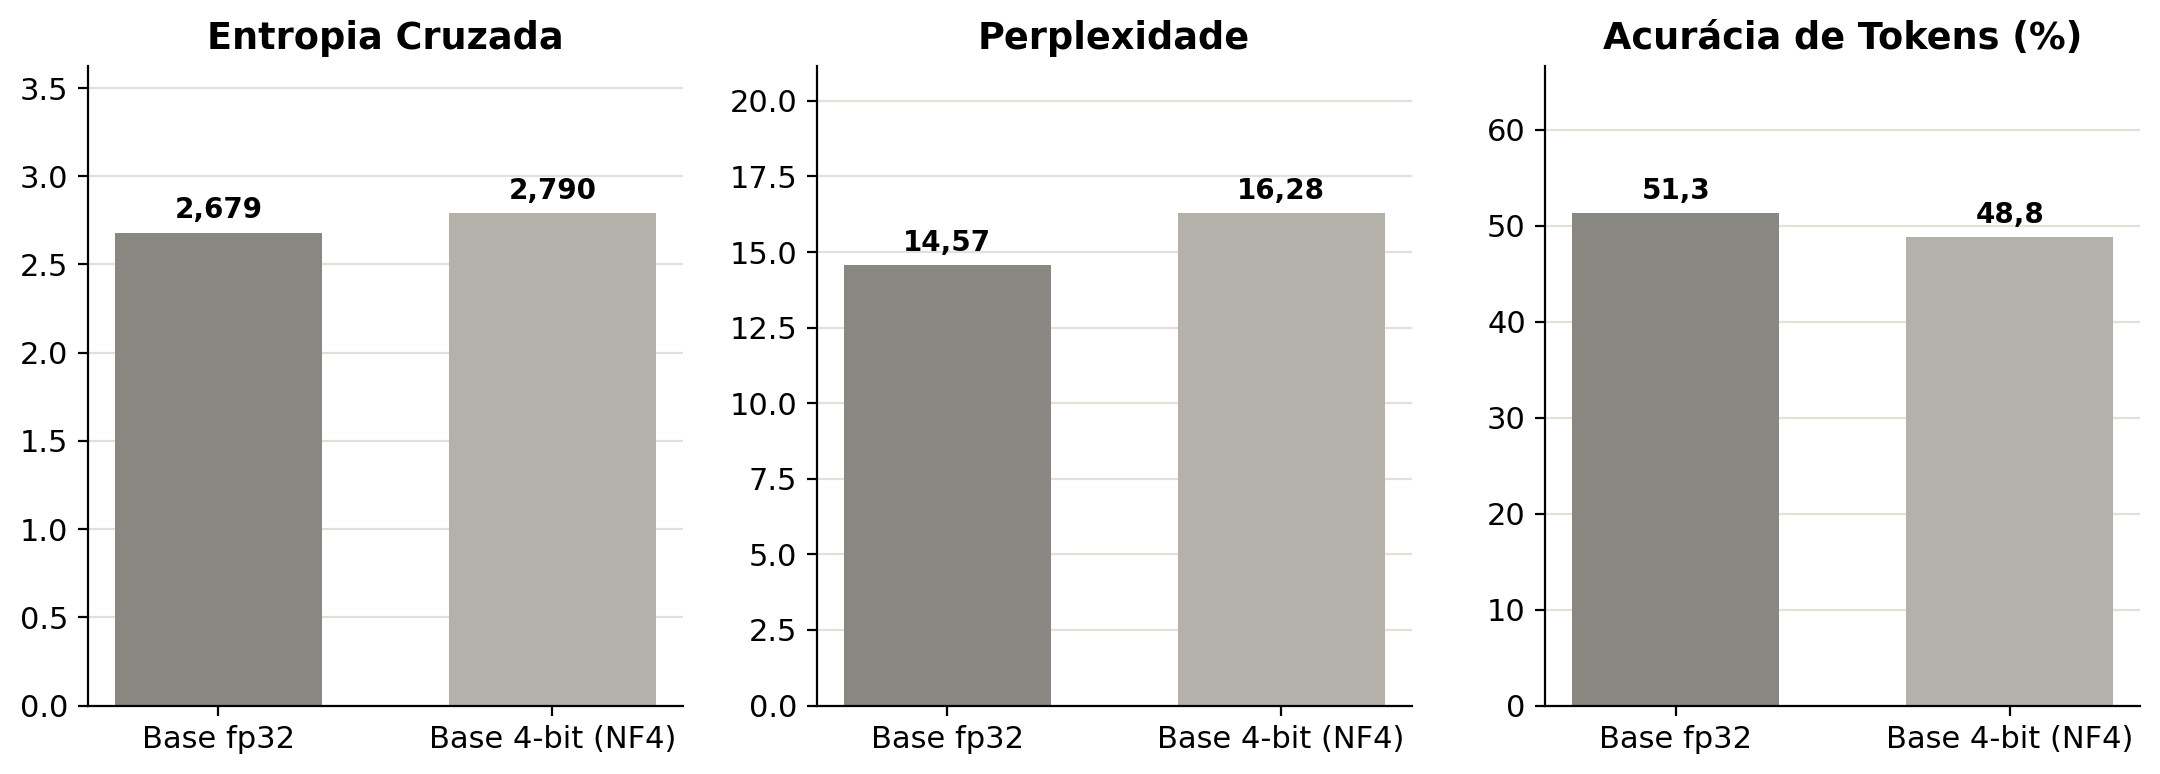
\includegraphics[width=\textwidth]{q3_quantizacao.png}
  \caption{Efeito da quantização NF4 sobre o modelo base, sem nenhum treino, no
  mesmo conjunto de avaliação da Questão 02.}
  \label{fig:q3-quant}
\end{figure}

\subsection{Resultados quantitativos}

Partindo do modelo quantizado (perplexidade 16,28), o QLoRA reduziu a perplexidade
sobre os tokens de resposta para 6,40 (queda de 60,7\%) e elevou a acurácia de
tokens de 48,78\% para 64,37\%. A Figura~\ref{fig:q3-metricas} posiciona esses
resultados ao lado dos da Questão 02, com os respectivos pontos de partida.

\begin{figure}[ht]
  \centering
  
\includegraphics[width=\textwidth]{q3_metricas.png}
  \caption{Métricas finais por técnica, com os dois baselines explicitados: o SFT
  completo parte da base em \texttt{fp32} e o QLoRA parte da base quantizada em 4
  bits. Métricas sobre os tokens de resposta do mesmo conjunto de avaliação.}
  \label{fig:q3-metricas}
\end{figure}

\subsection{Comparação com o ajuste fino completo}

O resultado central da questão está nas Figuras~\ref{fig:q3-params}
e~\ref{fig:q3-painel}: o QLoRA atingiu perplexidade final \emph{menor} que a do
ajuste fino completo (6,40 contra 7,49) atualizando 228 vezes menos parâmetros, com
pico de memória 5,5 vezes menor (1,77~GB contra 9,77~GB) e um artefato final de
8,7~MB contra cerca de 1~GB do modelo completo. Duas ressalvas contextualizam a
comparação: as taxas de aprendizado diferem (valor usual de cada técnica) e o QLoRA
parte de um baseline pior por causa da quantização, o que torna sua vantagem final
ainda mais notável.

A explicação é visível nas curvas de validação: enquanto o SFT completo entrou em
\textit{overfitting} na terceira época (Seção~\ref{sec:q2}), a perda de validação do
QLoRA caiu monotonicamente (0,929; 0,881; 0,878). Com apenas 1.728 exemplos de
treino, o adaptador de posto 16 age como uma regularização implícita: há menos graus
de liberdade para decorar o conjunto de treino.

\begin{figure}[ht]
  \centering
  
\includegraphics[width=0.9\textwidth]{q3_lora_params.png}
  \caption{Parâmetros atualizados por técnica, em escala logarítmica. A razão entre
  o SFT completo e o QLoRA do mesmo modelo é de 228 vezes.}
  \label{fig:q3-params}
\end{figure}

\begin{figure}[ht]
  \centering
  
\includegraphics[width=0.94\textwidth]{q3_painel_comparativo.png}
  \caption{Custo e qualidade das três variantes de pós-treino executadas sobre os
  mesmos dados. O QLoRA domina o SFT completo em perplexidade e memória; o modelo de
  1,5 bilhão quantizado obtém o melhor resultado geral.}
  \label{fig:q3-painel}
\end{figure}

A avaliação qualitativa, porém, inverte o ranking e completa o quadro: nas mesmas
dez perguntas da Questão 02, o QLoRA de 0,5 bilhão acertou apenas 2 (contra 6 do SFT
completo), falhando principalmente nos fatos fechados sobre o dataset. A leitura
conjunta é que atualizar todos os pesos memoriza conhecimento factual novo com mais
força, enquanto o adaptador aprende bem o formato e a distribuição das respostas,
mas retém menos fatos em um modelo desse porte. Afirmar superioridade do QLoRA
apenas pela perplexidade seria, portanto, uma conclusão incompleta.

\subsection{Experimento adicional: QLoRA no Qwen2.5-1.5B}

Atendendo ao item opcional do enunciado, a mesma configuração de QLoRA foi aplicada
ao \texttt{Qwen2.5-1.5B}. O modelo maior partiu de um baseline quantizado bem melhor
(perplexidade 10,28, inferior até à base de 0,5 bilhão em \texttt{fp32}) e terminou
com os melhores números do pós-treino: perplexidade 4,75, acurácia de tokens de
68,44\% e 5 acertos qualitativos em 10, treinando 0,28\% dos parâmetros em 2,75~GB
de VRAM. Escala e adaptação eficiente se mostraram complementares: o 1,5B com QLoRA
aproxima-se da qualidade factual do SFT completo gastando uma fração dos recursos.

\section{Discussão}
\label{sec:discussao}

\subsection{Pré-treino contra pós-treino}

As três questões ilustram dois regimes complementares de adaptação. O pré-treino
continuado (Questão 01) atua sobre a \emph{competência linguística} do modelo: sem
rótulos, apenas expondo-o ao corpus do domínio, reduziu a perplexidade em mais de
90\% e tornou suas gerações estilística e factualmente coerentes com o texto
administrativo do Piauí. Já o pós-treino (Questões 02 e 03) atua sobre o
\emph{comportamento} do modelo, ensinando-o a responder no formato
instrução/resposta. São objetivos distintos, e os resultados da Questão 01 mostram
que o ganho mais expressivo, em termos de modelagem de linguagem pura, vem da
exposição massiva ao domínio.

\subsection{SFT completo contra LoRA/QLoRA}

A comparação entre as Questões 02 e 03 é, em essência, uma análise de custo-benefício.
Os \textit{baselines} já coletados e o número de parâmetros treináveis
(Tabela~\ref{tab:comparativo}) deixam o trade-off evidente: o LoRA/QLoRA atualiza
0,44\% dos parâmetros e estimou treino cerca de 20 vezes mais rápido que o ajuste fino
completo no mesmo hardware. A hipótese a ser confirmada na execução final é a relatada
na literatura~\cite{hu2022lora,dettmers2023qlora}: que essa fração mínima de
parâmetros recupera a maior parte do ganho de qualidade do SFT completo, viabilizando
o ajuste em GPUs modestas.

\begin{table}[h]
  \centering
  \caption{Comparativo das três questões (valores ``depois'' de Q2 e Q3 pendentes de execução).}
  \label{tab:comparativo}
  \footnotesize
  \begin{tabularx}{\textwidth}{@{}l c c c c@{}}
    \toprule
    \textbf{Questão} & \textbf{Params. treinados} & \textbf{PPL antes} & \textbf{PPL depois} & \textbf{Acc. antes} \\
    \midrule
    01 -- Pré-treino   & 494M (100\%)   & 21,78 & \textbf{2,09} & 42,25\% \\
    02 -- SFT (full)   & 494M (100\%)   & 27,53 & \textit{em andamento} & 41,37\% \\
    03 -- LoRA/QLoRA   & 2,16M (0,44\%) & 34,51 & \textit{em andamento} & 38,42\% \\
    \bottomrule
  \end{tabularx}
\end{table}

\textbf{Ressalva de comparabilidade.} As perplexidades não são diretamente
comparáveis entre questões: a Questão 01 avalia sobre o DOMPI-2025, enquanto as
Questões 02 e 03 avaliam sobre o docentesDC; além disso, o \textit{baseline} da
Questão 03 é medido sobre o modelo quantizado em 4 bits. A comparação válida é sempre
\emph{antes contra depois dentro da mesma questão}.

\subsection{Limitações}

Cabe registrar as limitações do estudo. (i) As Questões 02 e 03 ainda não têm
métricas pós-treino, de modo que suas conclusões de qualidade são, por ora,
hipóteses fundamentadas no \textit{baseline} e na literatura, não em resultados
finais. (ii) A baixa perplexidade da Questão 01 é parcialmente atribuível à natureza
repetitiva do diário oficial, e não apenas à adaptação do modelo. (iii) Os pares de
QA gerados para o pós-treino têm qualidade desigual, conforme discutido na
Seção~\ref{sec:q2}, o que pode limitar o ganho do SFT antes das melhorias propostas.
(iv) Empregou-se um único modelo de 0,5~bilhão de parâmetros; o requisito opcional de
comparar modelos de tamanhos diferentes (p.\,ex.\ um Qwen2.5-1.5B via QLoRA) não foi
realizado.

\section{Considerações Finais}
\label{sec:consideracoes}

Este relatório documentou três experimentos de adaptação do \texttt{Qwen2.5-0.5B} ao
domínio público piauiense. A Questão 01, concluída integralmente, confirma sua
hipótese de forma robusta: o pré-treino continuado sobre o DOMPI-2025 reduziu a
perplexidade de 21,78 para 2,09 (queda de 90,4\%) e elevou a acurácia de previsão de
tokens de 42,25\% para 82,00\%, sem sinais de \textit{overfitting} e com clara
transformação qualitativa das gerações, que passaram de texto genérico para linguagem
administrativa autêntica do Piauí.

As Questões 02 (SFT completo) e 03 (LoRA/QLoRA) tiveram a metodologia, a geração dos
3.111 pares de instrução/resposta e a avaliação \textit{baseline} concluídas com
números reais, mas o treinamento foi interrompido por restrição de tempo de hardware
na tentativa local. Optou-se por reportar esse estado de forma transparente, sem
estimar métricas pós-treino. Os dados já evidenciam o principal trade-off entre as
duas técnicas: o LoRA/QLoRA atualiza apenas 0,44\% dos parâmetros e estimou treino
cerca de 20 vezes mais rápido que o ajuste fino completo.

\subsection{Caminho para conclusão das Questões 02 e 03}

Para fechar as duas questões pendentes, basta reexecutar os notebooks na GPU T4 do
Kaggle (o mesmo ambiente que viabilizou a Questão 01 em $\approx$4h40), aplicando os
ajustes já identificados:

\begin{enumerate}[leftmargin=2.2em]
  \item aplicar as três melhorias de qualidade dos pares de QA da
        Seção~\ref{sec:q2} (deduplicação, filtro de idioma, máscara de \textit{loss})
        e as perguntas de avaliação com nomes reais de professores;
  \item aplicar a correção do modo LoRA puro da Seção~\ref{sec:q3}
        (\texttt{enable\_input\_require\_grads});
  \item executar o treino, coletar as métricas pós-treino e preencher as células
        ``depois'' das Tabelas~\ref{tab:q2-baseline}, \ref{tab:q3-baseline}
        e~\ref{tab:comparativo}.
\end{enumerate}

Como o conjunto docentesDC é muito menor que o DOMPI-2025, estima-se que cada treino
leve apenas dezenas de minutos na T4, dominado pelo custo fixo de carregamento e
avaliação. A estrutura deste relatório já está preparada para receber esses números.

\subsection{Trabalhos futuros}

O trabalho da disciplina prevê ainda três frentes não cobertas por este relatório,
que dão sequência natural ao que foi construído: \textbf{(4)} destilação de
conhecimento de um modelo professor para um aluno; \textbf{(5)} uma aplicação de RAG
(\textit{Retrieval-Augmented Generation}) sobre o DOMPI-2025 ou o docentesDC, capaz
de recuperar fatos pontuais (CNPJ, CEP, e-mail) que o pré-treino não memoriza; e
\textbf{(6)} a inclusão de camadas de \textit{guardrails} sobre um dos modelos
desenvolvidos. A frente de RAG, em particular, complementa diretamente a limitação de
memorização factual observada no \textit{benchmark} da Questão 01.


\bibliographystyle{abntex2-alf}
\bibliography{refs}

\end{document}
